% ============================================================================
% CHAPTER 3  REQUIREMENTS SPECIFICATION
% ============================================================================

\chapter{Requirements Specification}
\label{chap:requirements}

% 
\section{Introduction}
\label{sec:req-intro}

This chapter describes what the MES-X Dependency Management system must do and
how well it must do it. The goal at this stage is to describe the expected
behavior independently of implementation choices, so the architecture and code
can later be measured against a clear baseline.

The requirements come from studying the manual workflow described in the
previous chapter, talking with developers and release engineers, and watching
traceability tasks being carried out in the MES X.0 environment. They cover
both what the system must do and the quality bar it must meet in daily use.


% 
\section{Functional Requirements}
\label{sec:functional-requirements}

The functional requirements define the main capabilities of the MES-X Dependency Management system.
They describe how the system processes Azure DevOps data to build a complete traceability view across work items, source code, and release information.

\begin{itemize}

\item \textbf{FR-01  Pull Request Resolution} \\
The system shall retrieve pull requests from Azure DevOps and associate them with their corresponding work items.  
This enables the system to establish a consistent link between work tracking elements and source control changes, which forms the entry point of the traceability pipeline.
\item \textbf{FR-02  Commit and Tag Contextualization} \\
The system shall extract commits linked to each pull request and add contextual information, including branch details and repository tags.  
This contextual information is required to determine the position of each change within the release lifecycle and to support release-level analysis.

\item \textbf{FR-03  Dependency Graph Construction} \\
The system shall construct a dependency graph starting from one or multiple root work items.  
It shall traverse all related entities through Azure DevOps relationships, including parent-child links, pull request associations, and commit references, in order to reconstruct the full dependency chain.

\item \textbf{FR-04  Aggregation and Decision Output} \\
The system shall aggregate all retrieved entities into a unified data model.  
This includes normalization of work items, pull requests, and commits, as well as removal of duplicates caused by multi-path traversal.  
The final output shall provide a structured view that supports release analysis and decision-making.

\item \textbf{FR-05  End-to-End Read-Only Traceability} \\
The system shall provide a complete traceability view across all relevant artifact levels: work items, pull requests, commits, branches, and tags.  
All interactions with Azure DevOps shall be strictly read-only, ensuring that no modification, creation, or deletion of external data is performed by the system.
\item \textbf{FR-06  Sprint-Based and Multi-Sprint Dependency Resolution} \\
The system shall support dependency analysis starting from one or more sprints, as well as from work items belonging to multiple sprints.  
It shall retrieve all related work items and trace their dependencies across pull requests, commits, and repository versions.

The system shall also identify the corresponding release versions associated with these work items in order to support validation of transitions between environments (e.g., development, pre-production, production).  
This enables the system to determine which changes are required to move a set of work items to the next environment.
\end{itemize}
\section{Non-Functional Requirements}
\label{sec:nonfunctional-requirements}

Non-functional requirements define the quality attributes that the system must respect to operate correctly in an industrial MES X.0 environment. They ensure that the system is not only functionally correct, but also performant, scalable, reliable, maintainable, and secure.

In this project, each non-functional requirement was directly translated into implementation decisions within the system architecture. Their validation was performed using a combination of unit tests, integration tests, runtime observation, and deployment-level verification.

% 
\subsection{Performance}

Performance ensures efficient dependency analysis even in large-scale distributed data.

\begin{itemize}

\item \textbf{NFR-PE-01  Graph Traversal Efficiency}:  
The system uses graph traversal strategies in the backend to explore relationships between work items, pull requests, and commits while avoiding redundant exploration. This requirement is supported by the Work Item and Commit services, which combine traversal logic with in-memory deduplication and visited-state management.

This requirement was verified through service-level tests and runtime observation of traversal behavior during dependency analysis.

\item \textbf{NFR-PE-02  API Call Optimization}:  
Azure DevOps API requests are optimized through batching and controlled concurrency. In particular, the backend uses the \texttt{p-limit} library to cap concurrent external calls in traceability-critical services such as work item traversal, commit resolution, and tag resolution.

This behavior was verified through code-level inspection of the concurrency control implementation, unit tests around the affected services, and runtime observation showing reduced request bursts and more stable execution.

\item \textbf{NFR-PE-03  Caching and Deduplication}:  
Processed entities are cached and deduplicated during traversal to avoid recomputation and repeated API calls. This is implemented through local caches, aggregation normalization, and repository-level deduplication utilities in the backend.

Its effectiveness was verified through repeated executions on identical inputs, which produced stable outputs with lower redundant processing.

\item \textbf{NFR-PE-04  Progressive Feedback}:  
Long-running operations provide streaming updates to the frontend, improving perceived responsiveness. This is implemented through Server-Sent Events, with a dedicated streaming service that emits progressive batches using the \texttt{text/event-stream} protocol.

This requirement was validated through end-to-end execution of batch analysis scenarios in which the frontend received progressive updates before full completion.

\end{itemize}

% 
\subsection{Scalability}

Scalability ensures the system can handle increasing data volume and repository complexity.

\begin{itemize}

\item \textbf{NFR-SC-01  Algorithmic Scalability}:  
The combination of graph traversal, caching, and controlled concurrency ensures that execution cost grows with the actual dependency graph size rather than with redundant repeated exploration.

This was verified through multi-root and sprint-based analysis scenarios involving multiple work items and repositories.

\item \textbf{NFR-SC-02  Microservices Architecture}:  
The system is divided into domain-focused backend services and modules, including Work Item, Pull Request, Commit, Sprint, Decision, and LLM modules. This modular NestJS architecture supports isolated evolution, clearer responsibilities, and future scaling of the processing pipeline.

This was verified during implementation by integrating new modules without redesigning the existing traceability flow.

\item \textbf{NFR-SC-03  Containerized Deployment}:  
Docker is used to package both backend and frontend applications, ensuring reproducible builds and deployment behavior across environments.

This was verified through the presence of Docker build scripts and Dockerfiles in both applications, as well as their integration into the delivery workflow.

\item \textbf{NFR-SC-04  Dapr Integration}:  
Dapr is used as an integration component for secret retrieval and distributed application support. In the current solution, it is concretely used to retrieve Azure DevOps secrets from the configured secret store and it prepares the platform for wider distributed-service evolution.

This was verified through the implemented backend integration based on \texttt{DaprClient} and the application configuration services.

\end{itemize}

% 
\subsection{Reliability}

Reliability ensures consistent system behavior under all execution conditions.

\begin{itemize}

\item \textbf{NFR-RE-01  Deterministic Output}:  
The system is designed to produce identical results for identical inputs regardless of execution order. This is supported by deterministic normalization, deduplication rules, and stable aggregation logic in the backend.

This requirement was verified through repeated runs using the same inputs and by checking that the resulting traceability outputs remained consistent.

\item \textbf{NFR-RE-02  Fault Isolation}:  
Failures in Azure DevOps API calls are isolated within the backend integration and service layers to avoid uncontrolled propagation across the whole application.

This is supported by dedicated service boundaries, exception handling, and structured logging in the NestJS backend.

\item \textbf{NFR-RE-03  Retry Mechanism}:  
Transient failures are handled using controlled recovery logic and guarded external-call handling while preserving partial processing whenever possible.

This was verified through service tests and runtime observation of backend behavior during unstable or partial-response situations.

\item \textbf{NFR-RE-04  Data Consistency}:  
All processed entities remain consistent across transformation and aggregation stages. This is supported by DTO-based contracts, typed mapping, and centralized aggregation logic.

This requirement was verified through unit tests, API checks, and frontend-backend consistency validation during traceability workflows.

\end{itemize}

% 
\subsection{Maintainability}

Maintainability ensures the system remains easy to evolve and extend.

\begin{itemize}

\item \textbf{NFR-MA-01  Modular Design}:  
Each module follows a modular design aligned with the Single Responsibility Principle, ensuring clear separation of concerns between traversal, commit processing, sprint handling, decision aggregation, and LLM review.

This was verified during development by the existence of dedicated backend modules and services with isolated responsibilities.

\item \textbf{NFR-MA-02  Clean Architecture}:  
Business logic, API integration, and data processing layers are separated to improve readability, testability, and long-term evolution. This separation is reflected in the NestJS service structure and in the dedicated configuration, integration, and utility layers.

This requirement was verified through code review, module boundaries, and the ability to test controllers and services independently.

\item \textbf{NFR-MA-03  Reusable Components}:  
Core services are designed to be reusable across multiple MES modules. Examples include shared streaming, logging, Azure DevOps integration, and aggregation utilities.

This was verified by reuse of common services across several backend domains.

\item \textbf{NFR-MA-04  Standardization}:  
Consistent naming conventions, DTO contracts, linting rules, and formatting rules are enforced across the codebase. This is supported by ESLint, Prettier, and typed DTO usage in both backend and frontend projects.

This requirement was verified through lint scripts, formatting scripts, and the standardized project structure used during implementation.

\end{itemize}

% 
\subsection{Security and Data Integrity}

Security ensures controlled and safe access to industrial data.

\begin{itemize}

\item \textbf{NFR-SE-01  Token-Based Authentication}:  
Azure DevOps access is secured using Personal Access Tokens whose secret names are provided through configuration and resolved at runtime from the secret store. The PAT is handled only by the backend and is never exposed to the frontend.

This requirement was verified through the implemented Azure DevOps connection service, which retrieves the secret through Dapr before creating the authenticated Azure DevOps client.

\item \textbf{NFR-SE-02  Frontend Route Protection}:  
The frontend includes a route-protection mechanism based on Vue Router metadata, a global \texttt{beforeEach} navigation guard, and an unauthorized fallback page. This mechanism allows views to be protected whenever \texttt{requiresAuth} is enabled.

This was verified through the implemented authentication and authorization flow in the frontend router and authentication store.

\item \textbf{NFR-SE-03  Secret Management}:  
Sensitive credentials are managed through secure configuration mechanisms using \texttt{ConfigService}, environment variables, and Dapr secret store integration.

This was verified through the backend configuration modules and runtime secret resolution logic.

\item \textbf{NFR-SE-04  Backend-Only External Access}:  
All communication with Azure DevOps is handled exclusively by the backend layer through dedicated integration services. The frontend communicates only with backend endpoints and does not directly call Azure DevOps.

This requirement was verified through the architecture, the implemented router/API flow, and the backend integration services.

\item \textbf{NFR-SE-05  Read-Only Policy}:  
The system is strictly read-only with respect to Azure DevOps, ensuring that no external artifacts are created, modified, or deleted during traceability analysis.

This was verified by reviewing the exposed backend functionality, which focuses on retrieval, traversal, enrichment, and aggregation only.

\end{itemize}
\subsection{Verification Scope}

This chapter defines the non-functional targets and the technical mechanisms
used to satisfy them. The concrete execution evidence (test outcomes,
deployment traces, and pipeline-level proof) is consolidated in the
Implementation chapter to avoid redundancy and keep this specification focused
on requirements and verification criteria.

\section{Use Case Model}
\label{sec:use-case-model}

The use case model shows how the actors interact with the system to carry out
traceability and analysis tasks. It complements the requirement lists with a
behavioral view of the system.

\subsection{Actors}
\label{subsec:actors}

The use case diagram highlights the two primary actors shown in the figure:
a Developer and an LLM Provider. The diagram is intended to make the main
workflow and intelligence flow visible at a glance.

\subsubsection{Developer and Release Engineer}

The primary user. Developers use the system to understand the impact of a work
item on the codebase. Release engineers use it to check release scope and
confirm whether changes sit on the correct side of a release boundary.

This actor starts analysis sessions, chooses the analysis mode, reviews
results, and uses the Decision Dashboard output to support release,
integration, and escalation decisions.

\subsubsection{LLM Provider}

An external AI service used by the system to review commits and generate
intelligent insights. This actor supports the "Review Commit with LLM" use
case and is shown in the diagram as a cross-cutting service.

\subsubsection{Additional Actors}

Other actors are part of the overall model but are not illustrated in this
view. The Administrator manages operational configuration and availability,
and Azure DevOps is the external data source for work items, pull requests,
commits, branches, and tags.

\subsection{Use Case Descriptions}
\label{subsec:use-cases}

The following use cases describe what the system does from each actor's
perspective.

\subsubsection{Work Item Use Cases}

\begin{itemize}
  \item \textbf{UC-01  Analyze Single Work Item}: The user provides one work item ID. The system traverses the full dependency graph, resolves related pull requests and commits, enriches commits with branch and tag context, and returns a complete normalized trace result.

  \item \textbf{UC-02  Analyze Multiple Work Items}: The user provides several work item IDs. The system traverses each root, merges and deduplicates the results, and returns one consolidated trace. This supports release scope analysis across a sprint or milestone.

  \item \textbf{UC-03  Stream Work Item Tasks}: The user starts a batch analysis session. The system streams resolved work item tasks progressively so progress is visible in real time, and items can be selected for further analysis before the full dataset has loaded.
\end{itemize}

\subsubsection{Pull Request Use Cases}

\begin{itemize}
  \item \textbf{UC-04  Retrieve Pull Request Work Items}: Given a pull request identifier, the system returns the work items formally linked to that PR on the Git side, along with the normalized PR summary including the repository name.
\end{itemize}

\subsubsection{Commit Use Cases}

\begin{itemize}
  \item \textbf{UC-05  Retrieve Commits by Work Item}: Given a work item ID, the system returns the deduplicated list of commits linked to that item, resolved through direct links and pull request expansion.

  \item \textbf{UC-06  Retrieve Commits by Pull Request}: Given a pull request ID, the system returns the list of commits merged as part of that PR.

  \item \textbf{UC-07  List Repository Branches and Tags}: Given a repository ID, the system returns the available branch and tag references needed to interpret commit positions.

  \item \textbf{UC-08  Resolve Commit Tag Context}: Given a repository and a commit, the system determines the most recent tag reachable from that commit on the relevant branch.

  \item \textbf{UC-09  Batch Resolve Commit Tag Context}: Given a repository and multiple commits, the system resolves the tag context of all specified commits in one operation to reduce API usage on large graphs.
\end{itemize}

\subsubsection{Aggregation and Decision Use Cases}

\begin{itemize}
  \item \textbf{UC-10  Generate Dependency View}: After a trace is complete, the system aggregates all collected data — work items, pull requests, commits, and tag context — into a single decision-ready view. Work items are grouped by completion state and repositories are classified by their commit position relative to the target release.

  \item \textbf{UC-11  Configure System}: The Administrator updates environment-level configuration, including Azure DevOps connection settings, API credential management, and deployment parameters.
\end{itemize}

\subsection{Use Case Diagram}
\label{subsec:use-case-diagram}

Figure~\ref{fig:usecase-diagram} shows the complete use case diagram, with the
primary actors and all eleven use cases.

\vspace{0.5em}
\hspace{0em}

\begin{figure}[H]
  \centering
  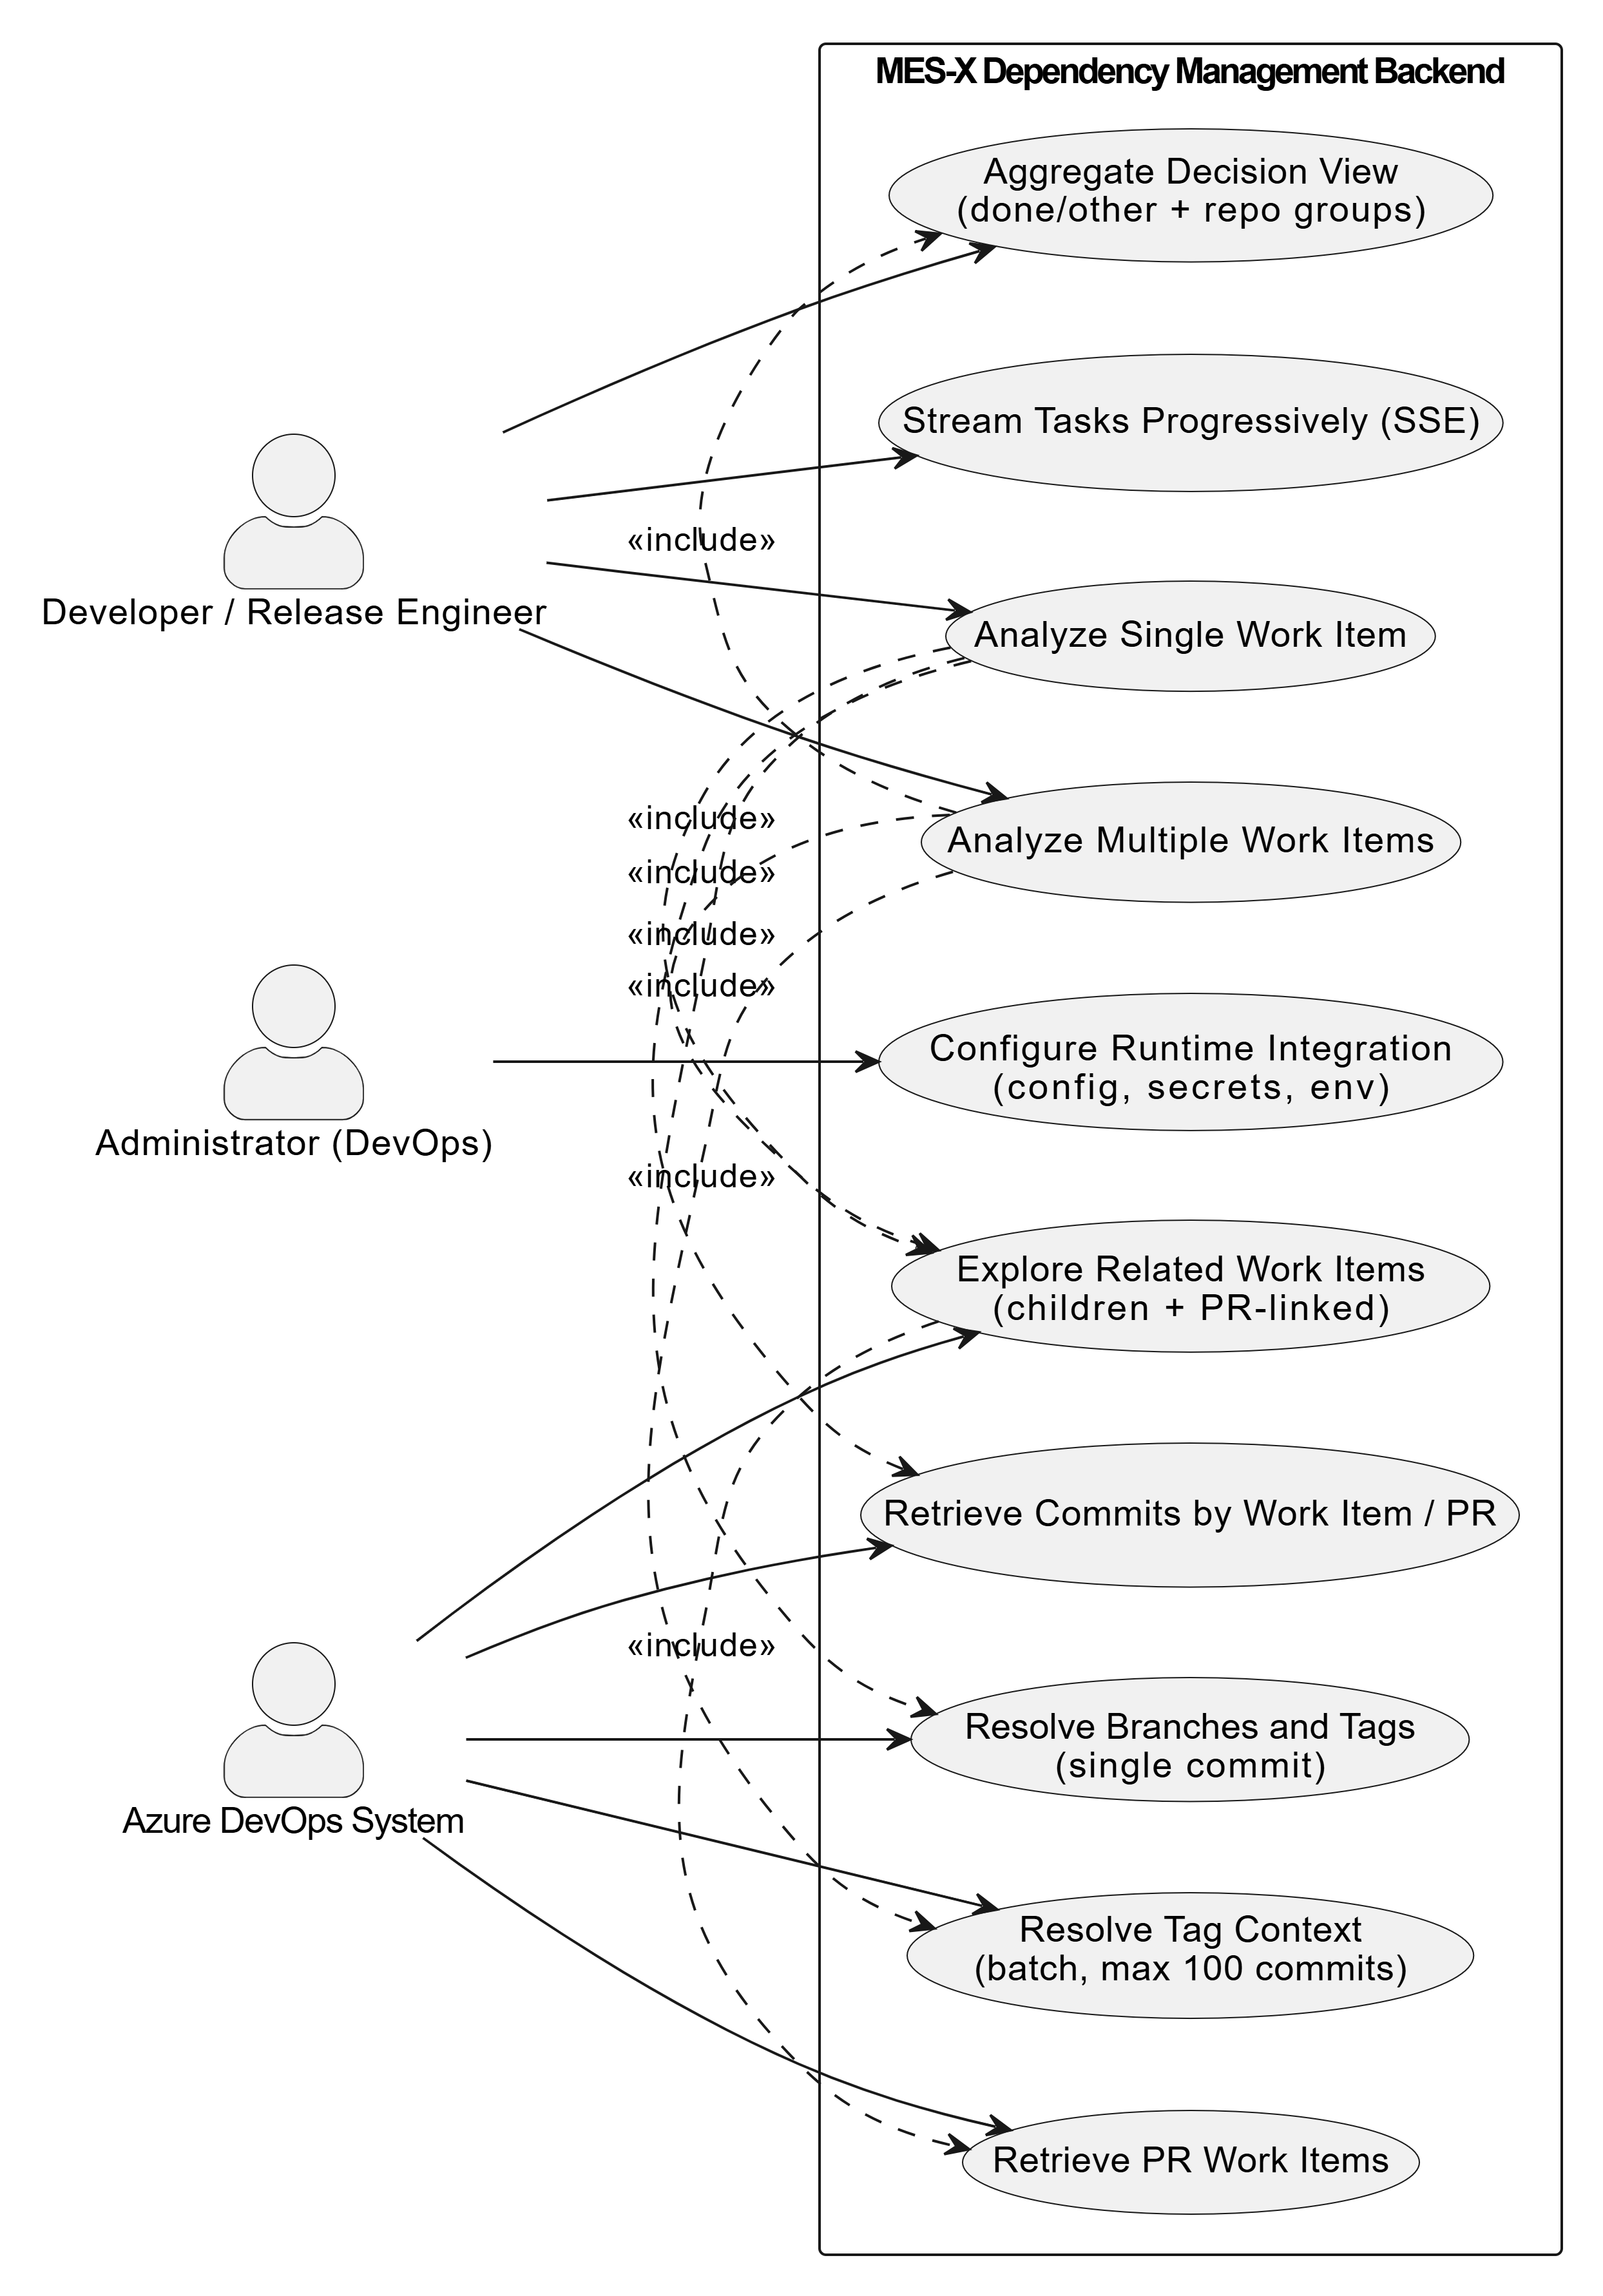
\includegraphics[width=1\textwidth,height=0.8\textheight,keepaspectratio]{img/archi/use_case.png}
  \caption{Use Case Diagram of the MES-X Dependency Management System.}
  \label{fig:usecase-diagram}
\end{figure}

\subsection{Scope Boundaries}
\label{subsec:scope-boundaries}

Two boundaries are worth stating clearly.

First, as set out in \textbf{FR-05}, all use cases are read-only. The system
does not create, modify, or delete anything in Azure DevOps. Azure DevOps
appears in the model only as a data source.

Second, notification and alerting features, mentioned in some internal notes as
possible future additions, are out of scope here. This specification covers
only the traceability and analysis capabilities described above.

% 
\section{Requirements Traceability Summary}
\label{sec:req-traceability}

Table~\ref{tab:req-traceability} shows how each functional requirement group
maps to a system component. This makes clear which part of the system is
responsible for which requirements, and creates the link between specification
and design.

\begin{table}[H]
  \centering
  \caption{Functional Requirements to System Component Traceability Matrix}
  \label{tab:req-traceability}
  \begin{tabular}{|p{4.5cm}|p{3cm}|p{5.5cm}|}
    \hline
    \textbf{Requirement Group} & \textbf{Requirement IDs} & \textbf{Responsible Component} \\
    \hline
    Pull Request Resolution & FR-01 & Pull Request Resolution Component \\
    \hline
    Commit and Tag Contextualization & FR-02 & Commit Aggregation Component \\
    \hline
    Dependency Graph Construction & FR-03 & Work Item Management Component \\
    \hline
    Aggregation and Decision Output & FR-04 & Decision Aggregation Component \\
    \hline
    End-to-End Read-Only Traceability & FR-05 & All components, Trace UI \\
    \hline
    Sprint-Based and Multi-Sprint Resolution & FR-06 & Sprint + Work Item + Commit Components \\
    \hline
  \end{tabular}
\end{table}

% 
\section{Conclusion}
\label{sec:req-conclusion}

This chapter set out the full requirements for the MES-X Dependency Management
system. The functional requirements cover five areas: work item traceability,
pull request resolution, commit enrichment, data aggregation, and analytical
reporting. The non-functional requirements set the bar for performance,
scalability, reliability, maintainability, and security. The use case model
translates those requirements into eleven concrete actor-system interactions.

Together, these requirements form the reference baseline for the rest of the
report. They define not just what the system must do, but the level of
performance, reliability, and maintainability expected of it in real use.

The next chapter presents the proposed architecture and explains how the chosen
design addresses these requirements through a layered structure and a
specialized traceability pipeline.